%Team Ramrod


\documentclass[pdftex, 11pt]{article}

\usepackage{setspace}
\usepackage[pdftex]{graphicx}
%\usepackage{url}

\newcommand{\HRule}{\rule{\linewidth}{0.5mm}}

%%\setlength{\textheight}{9in}
%%\setlength{\textwidth}{6in}

\addtolength{\oddsidemargin}{-0.375in}
\addtolength{\evensidemargin}{0.375in}
\addtolength{\textwidth}{0.5in}
\addtolength{\topmargin}{-.375in}
\addtolength{\textheight}{0.75in}


%\setlength{\oddsidemargin}{.25in}
%\setlength{\topmargin}{-.5in}  % changed from -.25 by RSR on 1/21/07

\hyphenation{itself}

\begin{document}



\begin{titlepage}
\begin{center}

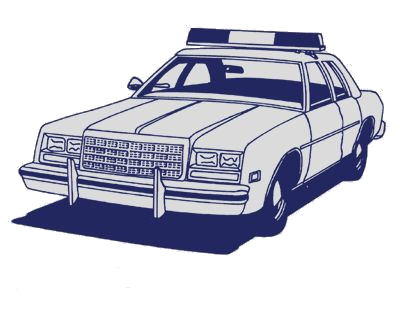
\includegraphics[width=0.5\textwidth]{./figures/logo.png}
\\[1cm]

\textsc{\LARGE TEAM RAMROD}\\[1.5cm]

\textsc{\Large Final Project Proposal}\\[0.5cm]

\HRule \\[0.4cm]
{\Huge \bfseries SNMP H4x0rZ}\\[0.4cm]
\HRule \\[1.5cm]

{\large
 \emph{Author:}\\
 Orion Miller\\
 Cameron Stearns\\
 Kellen Rogers\\
}

\vfill

{\large \today}

\end{center}
\end{titlepage}


\pagebreak

\setcounter{secnumdepth}{2}

\section{Goals}
We hope to demonstrate a known vulnerability of Simple Network Management 
Protocol (SNMP) over multiple anonymous systems.  As SNMP is commonly used 
to manage complex network resources, maintaining such a system is something 
that a small company may wish to outsource to a third party IT company.  
This company would likely have a direct VPN to access the SNMP servers and 
clients running on the remote system, which we will emulate as described below. 
The goal of this project is to highlight the insecurites of the SNMP protocol,
its common configurations and its negative effects of being a part of 
management systems (.e.g a hardware management system).

\section{Deliverables}

\begin{itemize}
\item Poster
  \subitem Abstract of final process
  \subitem Evaluation of attack successes, failures, and limitations
  \subitem Final network topology map (physical and logical)
  \subitem Genearl description of our process and methods

\item Demo
  \subitem Fully running version of the network topology %link to figure example
  \subitem Visual presentation of the results of several attacks

\item Write-Up
  \subitem Goals
  \subitem What we completed
  \subitem Dummy Corporate Network Explanation
  \subitem Explenation of SNMP Attacks
  \subitem How our tools were designed and how they work
  \subitem Network Configuration

\item Network Configuration
  \subitem Configuration files from each router
  \subitem Final Logical Network Topology
  \subitem Final Real Network Topology

\item SNMP Attack Tools
  \subitem SNMP tools that take advantage of SNMPv3  vulnerabilities
  \subitem Provide the source code for said tools

\end{itemize}

\section{Setup and Logistics}
In an overal structure for the completition of this project
we will need 3 main factors to be able to complete the project.
We need the Network setup, SNMP Servers and Clients and the
our written tools to actively exploit the vulnerabilities in
SNMP.

\subsection{Network}
In this project, we hope to create a network involving 3 autonomous 
systems [see figure].  We will configure a middle AS as a transit   %% add figure link
network, and run a VPN between the other two through it.

\begin{figure}
  \centering
  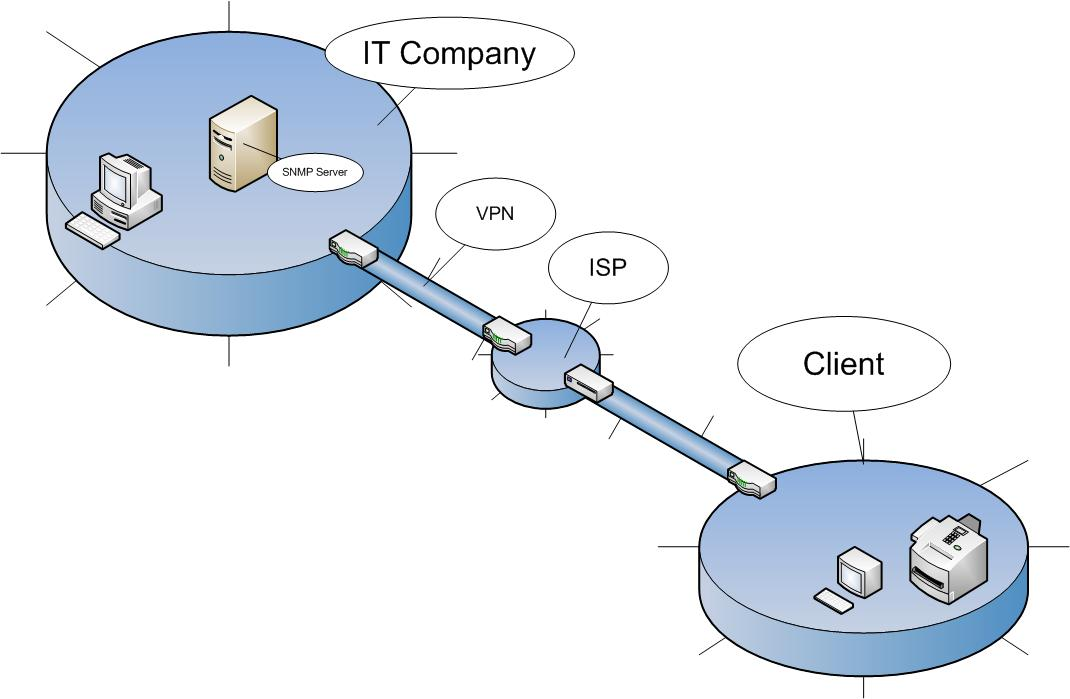
\includegraphics[width=0.95\textwidth, scale=1]{./figures/NetworkTopology.png}
  \caption{Proposed Network Topology}
\end{figure}

\subsection{SNMP}
Over this VPN, we will run the SNMP protocol, which has known 
implementation vulnerabilities as of SNMPv3. On the “IT” AS, we will 
run a server tasked with managing resources of the devices on our 
“Client” AS.  These resources will probably be things such as ink 
levels in a printer, or other easy to generate resources.

\subsection{Attacks}
When we attempt to exploit SNMP vulnerabilities, we will perform our 
attacks from several topological locations in our network.  The most 
obvious first place to try would be in either the “Client” or “IT” AS; 
however, we would also like to show results for attempts made from 
the “ISP” AS and other external locations.

\section{Deadlines}

\begin{center}
\begin{tabular}{l l}
  May 18 & Network Setup \& Functional \\
  May 20 & SNMP Servers \& Clients Functional \\
  May 25 & SNMP Exploits Tools Functional \\
  May 29 & Write-Up, Poster, \& Demo Completed \\
\end{tabular}
\end{center}




\end{document}
